% La recherche de similarité pour l'étude de la circulation des images

\subsection{Principe et méthodes de la recherche de similarité}
    \subsubsection{Des illustrations identiques ?}
    Un algorithme de recherche de similarité propose, à partir d'une image donnée, de trouver des images identiques ou similaires, sur la base de caractéristiques définies par un entraînement supervisé du modèle. L'utilisation de la vision artificielle pour la recherche d'images présentant des similitudes avec l'image donnée en requête présente une alternative intéressante à la recherche d'image basée sur les métadonnées de description, qui nécessite à la fois un bon référencement des images, et la capacité de l'utilisateur à formuler une requête qui lui permettra d'obtenir les résultats souhaités\footcite{farleyImageRetrievalConcepts2023}. Basées exclusivement sur les caractéristiques des images extraites par un réseau neuronal, les méthodes de \textit{similarity retrieval} permettent d'envisager la navigation de corpus massifs pour trouver des images identiques ou similaires, et présente ainsi un intérêt particulier pour les projets historiques s'intéressant aux copies, aux réemplois de motifs, et à la circulation des illustrations, des théories, des idées.
    
	L'entraînement d'un modèle de recherche de similarité nécessite un jeu de données annotées par les chercheurs. Pour la création dans un projet de données d'entraînement uniformes, il est ainsi nécessaire d'établir une définition claire de la similitude, qui prend en compte les limites de la détection par un modèle et répond aux attentes scientifiques des chercheurs. Le projet \vhs, porté sur la circulation des illustrations scientifiques dans les imprimés, prévoit l'intégration à sa chaîne de traitement de sources d'un modèle de \textit{similarity retrieval}, pour trouver dans l'ensemble des sources numérisées des images identiques, ou présentant des similitudes\footnote{Les préoccupations liées aux modèles de données pour une application intégrant la vision artificielle, détaillées dans la section \ref{detectionApp}, mentionnaient la nécessité de considérer les images extraites des numérisations par un algorithme de détection comme des entités à part entière, pour permettre le rattachement à leur numérisation et à la source dont elles sont issues. En considérant cette chaîne de traitement automatique, qui extrait les illustrations pour ensuite procéder à une recherche de similarité, ce lien des images au témoin est crucial, pour permettre d'établir une connexion entre les illustrations jugées identiques et les témoins qui les contiennent.}. Pour l'entraînement d'un tel modèle qui, comme explicité pour la détection d'objet, offre une vision foncièrement binaire de la similitude, des normes d'annotation ont été établies, suite à un dialogue entre les équipes impliquées dans le développement du modèle et les équipes de recherches, chargées de la création de la vérité de terrain. Ces normes permettent, notamment, de définir plusieurs niveaux de similitudes, allant d'illustrations identiques à illustrations différentes, qui établissent ainsi de manière tranchée ce que sont les similitudes entre images, figurant ainsi les attentes vis-à-vis du modèle de détection. Face aux limites de la technique, qui ne peut poser de regard critique sur les données traitées, une typologie précise des similitudes doit être définie pour annoter les images et classifier les sources, pour permettre un entraînement rigoureux et assurer de meilleures performances.
	
    \subsubsection{Médiation et métadonnées descriptives}
    La recherche de similarité se base sur des critères purement visuels pour regrouper des illustrations à partir d'une image envoyée en requête. Employée par un public de chercheurs possédant une expertise sur les sources, elle permet de mettre en avant des liens non-identifiés entre des documents du corpus, et de proposer une base pour une analyse plus poussée des motifs mis en avant. Ces méthodes sont ainsi profondément avantageuses pour des chercheurs aptes à appréhender les résultats, et à porter un regard critique sur les prédictions effectuées par un modèle. Cet aspect visuel des similarités soulignées présente cependant ses limites lorsqu'une application à destination du grand public est envisagée, et pour qui il est souhaitable de proposer une analyse sémantique, qui va au-delà des résultats du modèle, pour en faire plus qu'un outil de navigation de corpus. Pour la publication des données produites par un algorithme de recherche de similarité, il est nécessaire d'enrichir ces résultats de métadonnées, afin de proposer une contextualisation des images retournées. Sans considérer le grand public, l'objectif de ce type de traitements -- tout comme le partitionnement des données, évoqué dans la section suivante -- est de faire ressortir, pour les chercheurs, des illustrations inconnues, dont le lien avec l'image de requête n'avait pas été établi au préalable. Face à une source inconnue au chercheur, ce dernier doit donc trouver à sa disposition des métadonnées la replaçant dans son contexte pour permettre son analyse. Ces limites de la recherche par similarité impliquent ainsi de penser, en amont de la publication des résultats d'un projet exploitant ces méthodes, une étape manuelle de traitement et d'analyse des résultats par des chercheurs ayant une expertise sur les sources du corpus. Cette intervention critique sur les résultats obtenus par un traitement automatique permettent d'envisager la recherche de similarité dans une interface allant au-delà de l'outil de navigation, et de concevoir un véritable outil d'analyse et de médiation autour des sources du corpus étudié.

\subsection{Navigation de corpus par l'illustration}
Pour un projet tel que \vhs souhaitant mener une étude de la transmission et de la circulation des idées scientifiques, l'utilisation d'algorithmes de détection de similarité permet d'appréhender de manière automatique des tâches autrement fastidieuses de comparaison des illustrations présentes dans les ouvrages\footcite{kaouaImageCollationMatching2021}. Parmi les développements prévus par le projet, une application permettant l'extraction des illustrations dans des numérisations d'ouvrages, puis la recherche d'illustrations similaires dans toutes les sources du corpus devrait permettre l'automatisation de cette comparaison. L'une des fonctionnalités envisagées par le projet est la recherche de similarité systématique pour toutes les illustrations contenues dans une source sélectionnée, pour permettre aux utilisateurs de l'interface de naviguer aisément à travers les copies et reproductions des images dans les manuscrits et imprimés du corpus. Les résultats préliminaires du modèle utilisé\footcite{kaouaImageCollationMatching2021} (fig. \ref{fig:vhs_similarity}) témoigne de l'intérêt de l'usage de ce type d'algorithmes pour l'étude des phénomènes de copie entre les ouvrages dans un cadre chronologique et géographique vaste, avec la capacité d'identifier des remplois qu'une collation manuelle n'aurait pu souligner.

\begin{figure}[h]
	\hspace{1pt}
	\begin{subfigure}{0.5\linewidth}
		\centering
		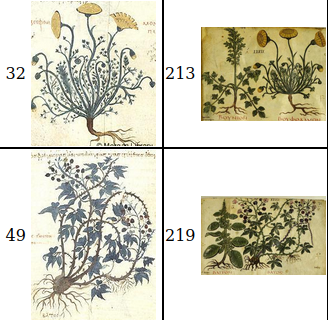
\includegraphics[width=7cm]{images/vhs_similarity.png}
	\end{subfigure}
	\hspace{1pt}
	\begin{subfigure}{0.5\linewidth}
		\centering
		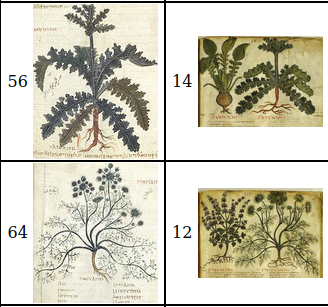
\includegraphics[width=7.5cm]{images/vhs_similarity2.png}
	\end{subfigure}
	\caption{Résultats préliminaires de recherche de similarité dans deux manuscrits du \textit{De Materia Medica} (\vhs)}
	\label{fig:vhs_similarity}
\end{figure}

\vhs hérite des méthodes et techniques développées dans le cadre du projet \enherit, dédié à l'exploration de corpus d'histoire de l'art par la vision artificielle, et particulièrement la détection de similarité. L'un des développements clés d'\enherit, appliqué notamment aux œuvres issues de l'atelier des Brueghel\footnote{Le jeu de données pour l'évaluation du modèle est constitué de 273 éléments dupliqués à travers 1587 tableaux attribués à Jan Brueghel et son atelier.}, est un algorithme de recherche de motifs identiques dans un corpus de peintures\footcite{shenDiscoveringVisualPatterns2019} affiné par apprentissage auto-supervisé\footnote{L'apprentissage auto-supervisé, à mi-chemin entre apprentissage supervisé et non-supervisé, est basé sur un jeu de données non annotées, pour lequel le modèle génère lui-même des étiquettes, qui varient à chaque itération.}. Si ce projet a constitué les bases techniques des projets \eida et \vhs, il n'a pas fait l'objet d'une application destinée à être utilisée de manière autonome par les historiens de l'art. \enherit témoigne cependant des applications possibles de la vision artificielle au traitement d'un corpus d'œuvres d'art, et offre des perspectives d'analyses automatiques portées, par exemple, sur la transmission de motifs dans un cadre temporel large ou sur la reproduction d'éléments spécifiques dans les ateliers. La recherche par similarité, au-delà d'une navigation par l'image dans des bases de données iconographiques, permet d'envisager une analyse de la tradition, de la transmission et des influences artistiques.

Le projet \eida prévoit également l'intégration d'algorithmes de recherche de similarité à sa chaîne de traitement des sources historiques, pour permettre la recherche de diagrammes similaires à partir d'un diagramme spécifique. Dans le cadre des objectifs scientifiques du projet, la notion de similarité pour des diagrammes astronomiques doit encore, à ce jour, être définie, pour déterminer les caractéristiques recherchées par l'algorithme. Bien qu'héritant des outils et pratiques d'\enherit, et malgré un lien avec le projet \vhs, les typologies à définir pour la similitude sont profondément différentes : les sources traitées, des diagrammes, ne peuvent être abordées avec des normes établies pour des œuvres d'art, ou pour des illustrations scientifiques, que l'aspect iconographique éloigne des diagrammes. La notion de copie, notamment, ne présente pas les mêmes enjeux pour le projet \eida, qui plutôt que de s'intéresser à la reproduction identique des diagrammes dans les manuscrits, porte son regard sur les différentes représentations existant à travers les traditions de modèles géométriques similaires. Les résultats préliminaires d'une recherche de similarité menée sur un jeu de données restreint de diagrammes\footnote{Réalisée par Tristan Dot et Sonat Baltaci en novembre 2022.} provenant d'éditions diverses de l'\textit{Almageste} de Ptolémée (fig. \ref{fig:eida_similarity}) semblent prometteurs pour le développement d'un outil qui permettrait aux chercheurs d'explorer la diversité des versions d'un même modèle à travers les sources du corpus.

\begin{figure}[h]
	\centering
	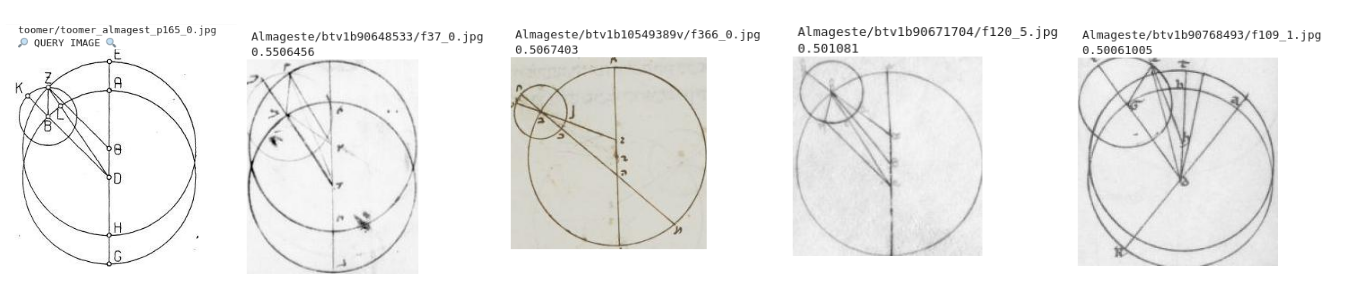
\includegraphics[width=16cm]{images/eida_similarity.png}
	\caption{Résultats préliminaires de recherche de similarité dans des diagrammes de l'\textit{Almageste} de Ptolémée (\eida)}
	\label{fig:eida_similarity}
\end{figure}